\documentclass{standalone}
\usepackage{tikz}
\usetikzlibrary{patterns, positioning}


\begin{document}
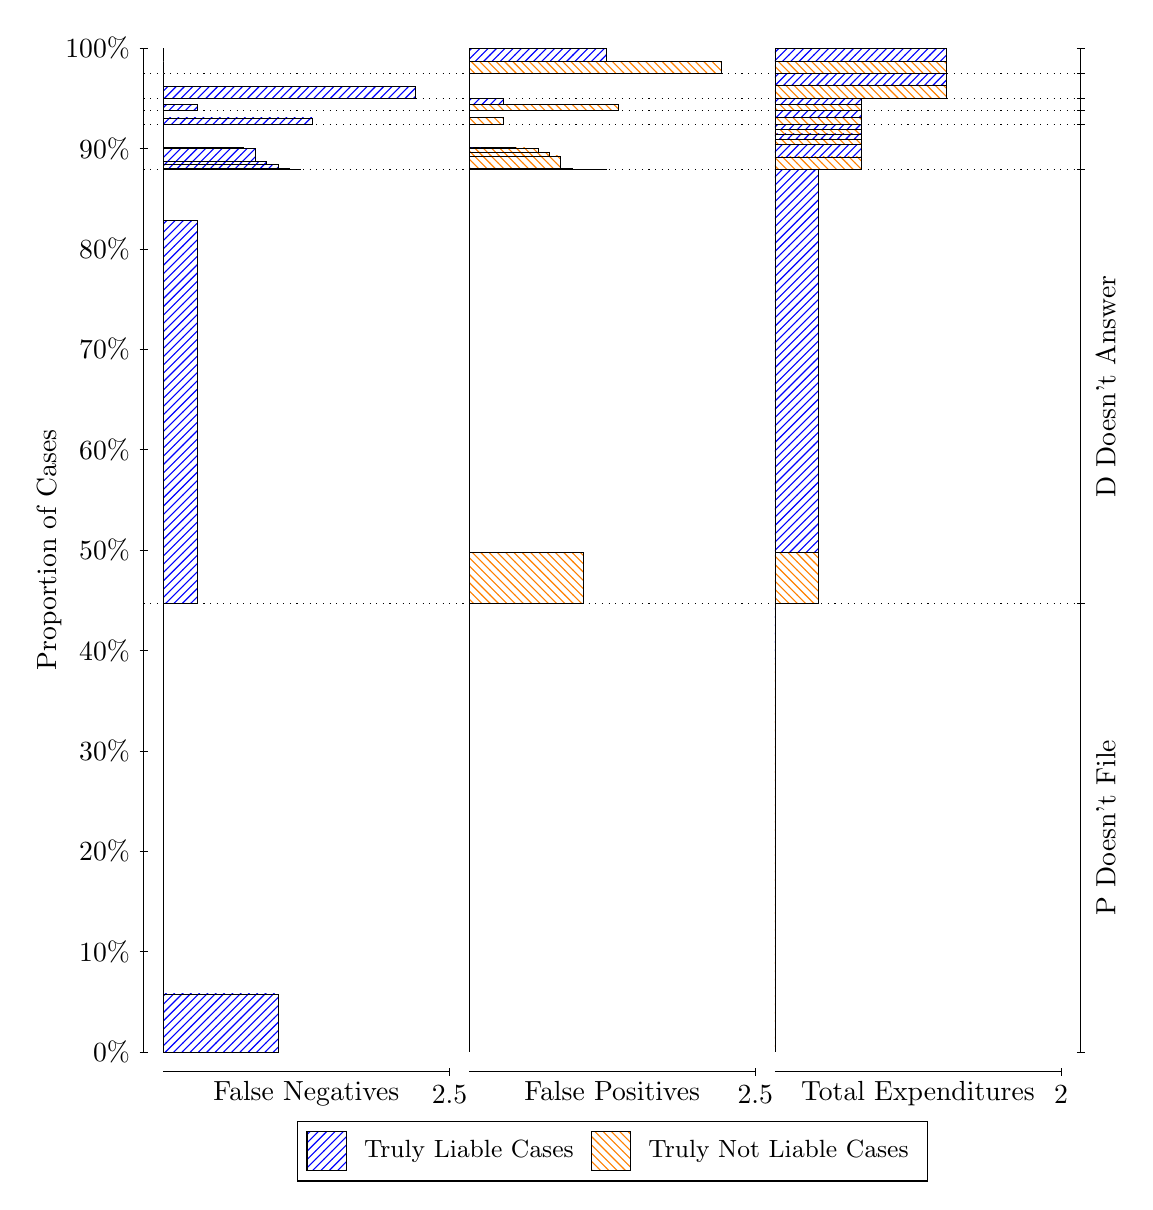
\begin{tikzpicture}
\draw[black, very thin] (1.5,1.75) -- (1.5,14.5);
\node[rotate=90, text=black, anchor=center] at (0.3, 8.125) {Proportion of Cases};
\draw[black, very thin] (1.45,1.75) -- (1.55,1.75);
\node[text=black, anchor=east] at (1.45, 1.75) {0\%};
\draw[black, very thin] (1.45,3.025) -- (1.55,3.025);
\node[text=black, anchor=east] at (1.45, 3.025) {10\%};
\draw[black, very thin] (1.45,4.3) -- (1.55,4.3);
\node[text=black, anchor=east] at (1.45, 4.3) {20\%};
\draw[black, very thin] (1.45,5.575) -- (1.55,5.575);
\node[text=black, anchor=east] at (1.45, 5.575) {30\%};
\draw[black, very thin] (1.45,6.85) -- (1.55,6.85);
\node[text=black, anchor=east] at (1.45, 6.85) {40\%};
\draw[black, very thin] (1.45,8.125) -- (1.55,8.125);
\node[text=black, anchor=east] at (1.45, 8.125) {50\%};
\draw[black, very thin] (1.45,9.4) -- (1.55,9.4);
\node[text=black, anchor=east] at (1.45, 9.4) {60\%};
\draw[black, very thin] (1.45,10.675) -- (1.55,10.675);
\node[text=black, anchor=east] at (1.45, 10.675) {70\%};
\draw[black, very thin] (1.45,11.95) -- (1.55,11.95);
\node[text=black, anchor=east] at (1.45, 11.95) {80\%};
\draw[black, very thin] (1.45,13.225) -- (1.55,13.225);
\node[text=black, anchor=east] at (1.45, 13.225) {90\%};
\draw[black, very thin] (1.45,14.5) -- (1.55,14.5);
\node[text=black, anchor=east] at (1.45, 14.5) {100\%};

\draw[black, very thin] (13.4,1.75) -- (13.4,14.5);
\draw[black, very thin] (13.35,1.75) -- (13.45,1.75);
\node[anchor=west] at (13.35, 1.75) {};
\draw[black, very thin] (13.35,7.4423) -- (13.45,7.4423);
\node[anchor=west] at (13.35, 7.4423) {};
\draw[black, very thin] (13.35,12.955) -- (13.45,12.955);
\node[anchor=west] at (13.35, 12.955) {};
\draw[black, very thin] (13.35,13.527) -- (13.45,13.527);
\node[anchor=west] at (13.35, 13.527) {};
\draw[black, very thin] (13.35,13.706) -- (13.45,13.706);
\node[anchor=west] at (13.35, 13.706) {};
\draw[black, very thin] (13.35,13.863) -- (13.45,13.863);
\node[anchor=west] at (13.35, 13.863) {};
\draw[black, very thin] (13.35,14.179) -- (13.45,14.179);
\node[anchor=west] at (13.35, 14.179) {};
\draw[black, very thin] (13.35,14.5) -- (13.45,14.5);
\node[anchor=west] at (13.35, 14.5) {};

\draw[black, very thin, pattern color=blue, pattern=north east lines] (1.75,1.75) rectangle (3.2033,2.4865);
\draw[black, very thin, pattern color=orange, pattern=north west lines] (1.75,2.4865) rectangle (1.75,7.4423);
\draw[black, very thin, pattern color=blue, pattern=north east lines] (1.75,7.4423) rectangle (2.186,12.308);
\draw[black, very thin, pattern color=orange, pattern=north west lines] (1.75,12.308) rectangle (1.75,12.955);
\draw[black, very thin, pattern color=blue, pattern=north east lines] (1.75,12.955) rectangle (3.494,12.963);
\draw[black, very thin, pattern color=blue, pattern=north east lines] (1.75,12.963) rectangle (3.3487,12.973);
\draw[black, very thin, pattern color=blue, pattern=north east lines] (1.75,12.973) rectangle (3.2033,13.018);
\draw[black, very thin, pattern color=blue, pattern=north east lines] (1.75,13.018) rectangle (3.058,13.019);
\draw[black, very thin, pattern color=blue, pattern=north east lines] (1.75,13.019) rectangle (3.058,13.065);
\draw[black, very thin, pattern color=blue, pattern=north east lines] (1.75,13.065) rectangle (2.9127,13.222);
\draw[black, very thin, pattern color=blue, pattern=north east lines] (1.75,13.222) rectangle (2.7673,13.234);
\draw[black, very thin, pattern color=blue, pattern=north east lines] (1.75,13.234) rectangle (2.622,13.239);
\draw[black, very thin, pattern color=blue, pattern=north east lines] (1.75,13.239) rectangle (2.4767,13.239);
\draw[black, very thin, pattern color=blue, pattern=north east lines] (1.75,13.239) rectangle (2.3313,13.24);
\draw[black, very thin, pattern color=orange, pattern=north west lines] (1.75,13.24) rectangle (1.75,13.527);
\draw[black, very thin, pattern color=blue, pattern=north east lines] (1.75,13.527) rectangle (3.6393,13.612);
\draw[black, very thin, pattern color=orange, pattern=north west lines] (1.75,13.612) rectangle (1.75,13.706);
\draw[black, very thin, pattern color=blue, pattern=north east lines] (1.75,13.706) rectangle (2.186,13.788);
\draw[black, very thin, pattern color=orange, pattern=north west lines] (1.75,13.788) rectangle (1.75,13.863);
\draw[black, very thin, pattern color=blue, pattern=north east lines] (1.75,13.863) rectangle (4.9473,14.011);
\draw[black, very thin, pattern color=orange, pattern=north west lines] (1.75,14.011) rectangle (1.75,14.179);
\draw[black, very thin, pattern color=orange, pattern=north west lines] (1.75,14.179) rectangle (1.75,14.328);
\draw[black, very thin, pattern color=blue, pattern=north east lines] (1.75,14.328) rectangle (1.75,14.5);
\draw[black, very thin, pattern color=orange, pattern=north west lines] (5.6333,1.75) rectangle (5.6333,6.7057);
\draw[black, very thin, pattern color=blue, pattern=north east lines] (5.6333,6.7057) rectangle (5.6333,7.4423);
\draw[black, very thin, pattern color=orange, pattern=north west lines] (5.6333,7.4423) rectangle (7.0867,8.09);
\draw[black, very thin, pattern color=blue, pattern=north east lines] (5.6333,8.09) rectangle (5.6333,12.955);
\draw[black, very thin, pattern color=orange, pattern=north west lines] (5.6333,12.955) rectangle (7.3773,12.956);
\draw[black, very thin, pattern color=orange, pattern=north west lines] (5.6333,12.956) rectangle (7.232,12.957);
\draw[black, very thin, pattern color=orange, pattern=north west lines] (5.6333,12.957) rectangle (7.0867,12.962);
\draw[black, very thin, pattern color=orange, pattern=north west lines] (5.6333,12.962) rectangle (6.9413,12.974);
\draw[black, very thin, pattern color=orange, pattern=north west lines] (5.6333,12.974) rectangle (6.796,13.13);
\draw[black, very thin, pattern color=orange, pattern=north west lines] (5.6333,13.13) rectangle (6.6507,13.177);
\draw[black, very thin, pattern color=orange, pattern=north west lines] (5.6333,13.177) rectangle (6.5053,13.222);
\draw[black, very thin, pattern color=orange, pattern=north west lines] (5.6333,13.222) rectangle (6.36,13.232);
\draw[black, very thin, pattern color=orange, pattern=north west lines] (5.6333,13.232) rectangle (6.2147,13.242);
\draw[black, very thin, pattern color=blue, pattern=north east lines] (5.6333,13.242) rectangle (5.924,13.243);
\draw[black, very thin, pattern color=blue, pattern=north east lines] (5.6333,13.243) rectangle (5.7787,13.243);
\draw[black, very thin, pattern color=blue, pattern=north east lines] (5.6333,13.243) rectangle (5.6333,13.527);
\draw[black, very thin, pattern color=orange, pattern=north west lines] (5.6333,13.527) rectangle (6.0693,13.62);
\draw[black, very thin, pattern color=blue, pattern=north east lines] (5.6333,13.62) rectangle (5.6333,13.706);
\draw[black, very thin, pattern color=orange, pattern=north west lines] (5.6333,13.706) rectangle (7.5227,13.781);
\draw[black, very thin, pattern color=blue, pattern=north east lines] (5.6333,13.781) rectangle (6.0693,13.863);
\draw[black, very thin, pattern color=orange, pattern=north west lines] (5.6333,13.863) rectangle (5.6333,14.031);
\draw[black, very thin, pattern color=blue, pattern=north east lines] (5.6333,14.031) rectangle (5.6333,14.179);
\draw[black, very thin, pattern color=orange, pattern=north west lines] (5.6333,14.179) rectangle (8.8307,14.328);
\draw[black, very thin, pattern color=blue, pattern=north east lines] (5.6333,14.328) rectangle (7.3773,14.5);
\draw[black, very thin, pattern color=orange, pattern=north west lines] (9.5167,1.75) rectangle (9.5167,6.7057);
\draw[black, very thin, pattern color=blue, pattern=north east lines] (9.5167,6.7057) rectangle (9.5167,7.4423);
\draw[black, very thin, pattern color=orange, pattern=north west lines] (9.5167,7.4423) rectangle (10.062,8.09);
\draw[black, very thin, pattern color=blue, pattern=north east lines] (9.5167,8.09) rectangle (10.062,12.955);
\draw[black, very thin, pattern color=orange, pattern=north west lines] (9.5167,12.955) rectangle (10.607,13.117);
\draw[black, very thin, pattern color=blue, pattern=north east lines] (9.5167,13.117) rectangle (10.607,13.279);
\draw[black, very thin, pattern color=orange, pattern=north west lines] (9.5167,13.279) rectangle (10.607,13.345);
\draw[black, very thin, pattern color=blue, pattern=north east lines] (9.5167,13.345) rectangle (10.607,13.409);
\draw[black, very thin, pattern color=orange, pattern=north west lines] (9.5167,13.409) rectangle (10.607,13.468);
\draw[black, very thin, pattern color=blue, pattern=north east lines] (9.5167,13.468) rectangle (10.607,13.527);
\draw[black, very thin, pattern color=orange, pattern=north west lines] (9.5167,13.527) rectangle (10.607,13.62);
\draw[black, very thin, pattern color=blue, pattern=north east lines] (9.5167,13.62) rectangle (10.607,13.706);
\draw[black, very thin, pattern color=orange, pattern=north west lines] (9.5167,13.706) rectangle (10.607,13.781);
\draw[black, very thin, pattern color=blue, pattern=north east lines] (9.5167,13.781) rectangle (10.607,13.863);
\draw[black, very thin, pattern color=orange, pattern=north west lines] (9.5167,13.863) rectangle (11.697,14.031);
\draw[black, very thin, pattern color=blue, pattern=north east lines] (9.5167,14.031) rectangle (11.697,14.179);
\draw[black, very thin, pattern color=orange, pattern=north west lines] (9.5167,14.179) rectangle (11.697,14.328);
\draw[black, very thin, pattern color=blue, pattern=north east lines] (9.5167,14.328) rectangle (11.697,14.5);
\draw[black, dotted] (1.5,7.4423) -- (13.4,7.4423);
\draw[black, dotted] (1.5,12.955) -- (13.4,12.955);
\draw[black, dotted] (1.5,13.527) -- (13.4,13.527);
\draw[black, dotted] (1.5,13.706) -- (13.4,13.706);
\draw[black, dotted] (1.5,13.863) -- (13.4,13.863);
\draw[black, dotted] (1.5,14.179) -- (13.4,14.179);
\draw[black, very thin] (1.75,1.5) -- (5.3833,1.5);
\node[text=black, anchor=north] at (3.5667, 1.5) {False Negatives};
\draw[black, very thin] (5.3833,1.45) -- (5.3833,1.55);
\node[text=black, anchor=north] at (5.3833, 1.45) {2.5};

\draw[black, very thin] (5.6333,1.5) -- (9.2667,1.5);
\node[text=black, anchor=north] at (7.45, 1.5) {False Positives};
\draw[black, very thin] (9.2667,1.45) -- (9.2667,1.55);
\node[text=black, anchor=north] at (9.2667, 1.45) {2.5};

\draw[black, very thin] (9.5167,1.5) -- (13.15,1.5);
\node[text=black, anchor=north] at (11.333, 1.5) {Total Expenditures};
\draw[black, very thin] (13.15,1.45) -- (13.15,1.55);
\node[text=black, anchor=north] at (13.15, 1.45) {2};

\node[text=black, centered, rotate=90] at (13.72, 4.5961) {P Doesn't File};
\node[text=black, centered, rotate=90] at (13.72, 10.199) {D Doesn't Answer};






\draw (7.449999999999999,1.5) node[draw=none] (baseCoordinate) {};
\begin{scope}[align=center]
        \matrix[scale=0.5, draw=black, below=0.5cm of baseCoordinate, nodes={draw}, column sep=0.1cm]{
            \node[rectangle, draw, minimum width=0.5cm, minimum height=0.5cm, pattern color=blue, pattern=north east lines] {}; &
            \node[draw=none, font=\small, text=black] (B) {Truly Liable Cases}; &
            \node[rectangle, draw, minimum width=0.5cm, minimum height=0.5cm, pattern color=orange, pattern=north west lines] {}; &
            \node[draw=none, font=\small, text=black] (B) {Truly Not Liable Cases}; \\
            };
\end{scope}

\end{tikzpicture}
\end{document}